\documentclass{standalone}
\usepackage{tikz}
\usepackage{ctex,siunitx}
\setCJKmainfont{Noto Serif CJK SC}
\usepackage{tkz-euclide}
\usepackage{amsmath}
\usetikzlibrary{patterns, calc,3d}
\usetikzlibrary {decorations.pathmorphing,decorations.pathreplacing,decorations.shapes,}
\tikzset{label style/.append style={font=\small}}
\begin{document}
\small
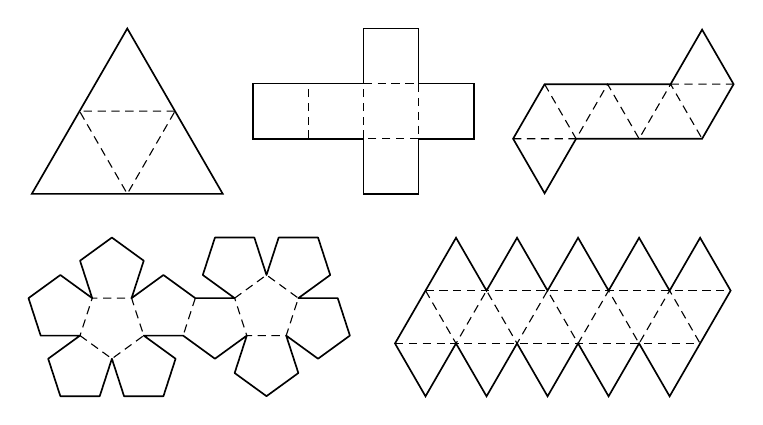
\begin{tikzpicture}[>=latex,scale=1.0]
  \begin{scope}
    \draw[semithick,line join=round](0,0)--++(180:0.5)--++(108:0.5)--++(36:0.5)--++(-36:0.5)--++(108:0.5)--++(36:0.5)--++(-36:0.5)--++(-108:0.5)--++(36:0.5)--++(-36:0.5)coordinate(n1)--++(0:0.5)coordinate(n2)--++(144:0.5)--++(72:0.5)--++(0:0.5)--++(-72:0.5)--++(72:0.5)--++(0:0.5)--++(-72:0.5)--++(-144:0.5)--++(0:0.5)--++(-72:0.5)--++(-144:0.5)--++(144:0.5)--++(-72:0.5)--++(-144:0.5)--++(144:0.5)--++(72:0.5)--++(-144:0.5)--++(144:0.5)--++(180:0.5)--++(-36:0.5)--++(-108:0.5)--++(180:0.5)--++(108:0.5)--++(-108:0.5)--++(180:0.5)--++(108:0.5)--cycle;
    \draw[densely dashed]
    (0,0)--++(-36:0.5)--++(36:0.5)--++(108:0.5)--++(180:0.5)--cycle
    (n1)--++(-108:0.5)
    (n2)--++(36:0.5)--++(-36:0.5)--++(-108:0.5)--++(180:0.5)--cycle;
  \end{scope}
  \begin{scope}[xshift=4cm,yshift=-1mm,scale=1.55]
    \draw[semithick](0,0)--(60:0.5)
    \foreach \x in {1,...,5} {--++(60:0.5)--++(-60:0.5)}--++(-120:0.5)
    \foreach \x in {1,...,5} {--++(-120:0.5)--++(120:0.5)}--cycle;
    \draw[densely dashed](0,0)--(2.5,0)(60:0.5)--++(2.5,0);
    \draw[densely dashed](60:0.5)--++(-60:0.5)--++(60:0.5)--++(-60:0.5)--++(60:0.5)--++(-60:0.5)--++(60:0.5)--++(-60:0.5)--++(60:0.5)--++(-60:0.5);
  \end{scope}
  \begin{scope}[xshift=2.2cm,yshift=2.5cm,scale=0.7]
    \draw[semithick](0,0)--++(2,0)--++(0,-1)--++(1,0)--++(0,1)--++(1,0)--++(0,1)--++(-1,0)--++(0,1)--++(-1,0)--++(0,-1)--++(-2,0)--cycle;
    \draw[densely dashed](2,0)rectangle(3,1)(1,0)--(1,1);
  \end{scope}
  \begin{scope}[xshift=5.5cm,yshift=2.5cm,scale=0.8]
    \draw[semithick](0,0)--(60:1)--++(2,0)--++(60:1)--++(-60:1)--++(-120:1)--++(-2,0)--++(-120:1)--cycle;
    \draw[densely dashed](0,0)--(1,0)(60:1)--++(-60:1)--++(60:1)--++(-60:1)--++(60:1)--++(-60:1)([xshift=2cm]60:1)--++(1,0);
  \end{scope}
  \begin{scope}[xshift=6mm,yshift=2.5cm,scale=1.4]
    \draw[semithick](-30:1)--(-150:1)--(90:1)--cycle;
    \draw[densely dashed](30:0.5)--(150:0.5)--(-90:0.5)--cycle;
  \end{scope}
\end{tikzpicture}
\end{document}